\documentclass[tikz]{standalone}

\usetikzlibrary{
    chains,
    positioning,
    arrows.meta,
    decorations.pathreplacing,
    calc,
    fit,
    shapes.geometric
}

\begin{document}

% Adapted from
% https://tex.stackexchange.com/questions/468410/tikz-drawing-layer-by-layer

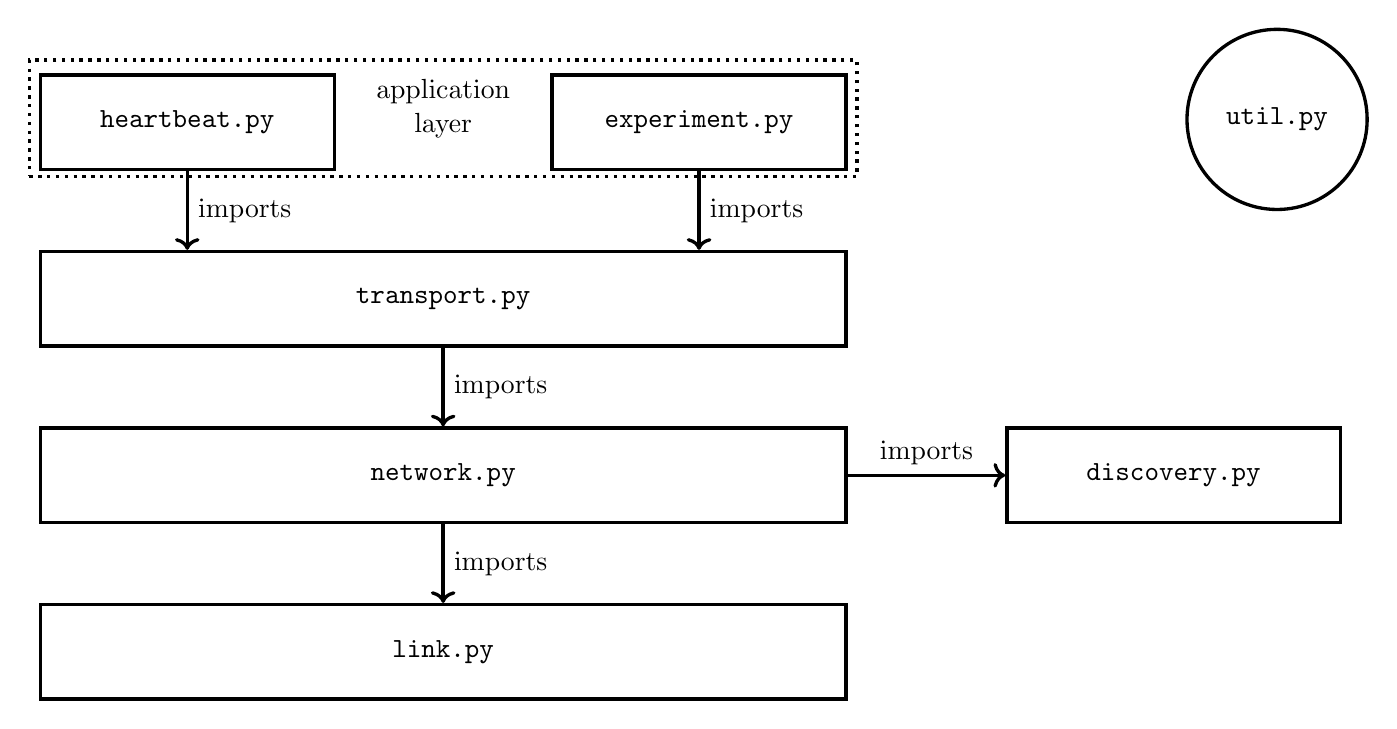
\begin{tikzpicture}[
    node distance = -0.5mm and 0mm,
    start chain = going below,
    module/.style args = {#1}{
        rectangle, draw, very thick,
        text width=3.5cm, align=center,
        minimum height=12mm,
        on chain
    },
]
    
    \node (transport) [module, text width=10cm] {\texttt{transport.py}};
    
    \node (heartbeat) [module, above right=1cm and 0cm of transport.north west] {\texttt{heartbeat.py}};
    \draw[very thick,->] (heartbeat) -- node[right] {imports} (heartbeat |- transport.north);
    
    \node (experiment) [module, above left=1cm and 0cm of transport.north east] {\texttt{experiment.py}};
    \draw[very thick,->] (experiment) -- node[right] {imports} (experiment |- transport.north);
    
    \node (app) [module, dotted, fit=(heartbeat)(experiment)] {application\\layer};
    
    \node (network) [module, below right=1cm and 0cm of transport.south west, text width=10cm] {\texttt{network.py}};
    \draw[very thick,->] (transport) -- node[right] {imports} (transport |- network.north);
    
    \node (discovery) [module, right=2cm of network, text width=4cm] {\texttt{discovery.py}};
    \draw[very thick,->] (network) -- node[above] {imports} (discovery);
    
    \node (link) [module, below right=1cm and 0cm of network.south west, text width=10cm] {\texttt{link.py}};
    \draw[very thick,->] (network) -- node[right] {imports} (network |- link.north);
    
    \node [module,circle,draw,below left,text width=2cm] at (current bounding box.north east) {\texttt{util.py}};
\end{tikzpicture}

\end{document}
